% !TEX root = ../../../main.tex
%

\chapter{Cablaggio Strutturato}


\section{Planimetrie}
Si riportano di seguito le planimetrie piano terreno (\autoref{fig:planimetria-terreno}) e dei successivi piani
dell'edificio (\autoref{fig:planimetria-1}) opportunamente annotate e dimensionate.
Le quote sono approssimative in quanto non fornite nelle specifiche originali.

\begin{figure}[ht]
    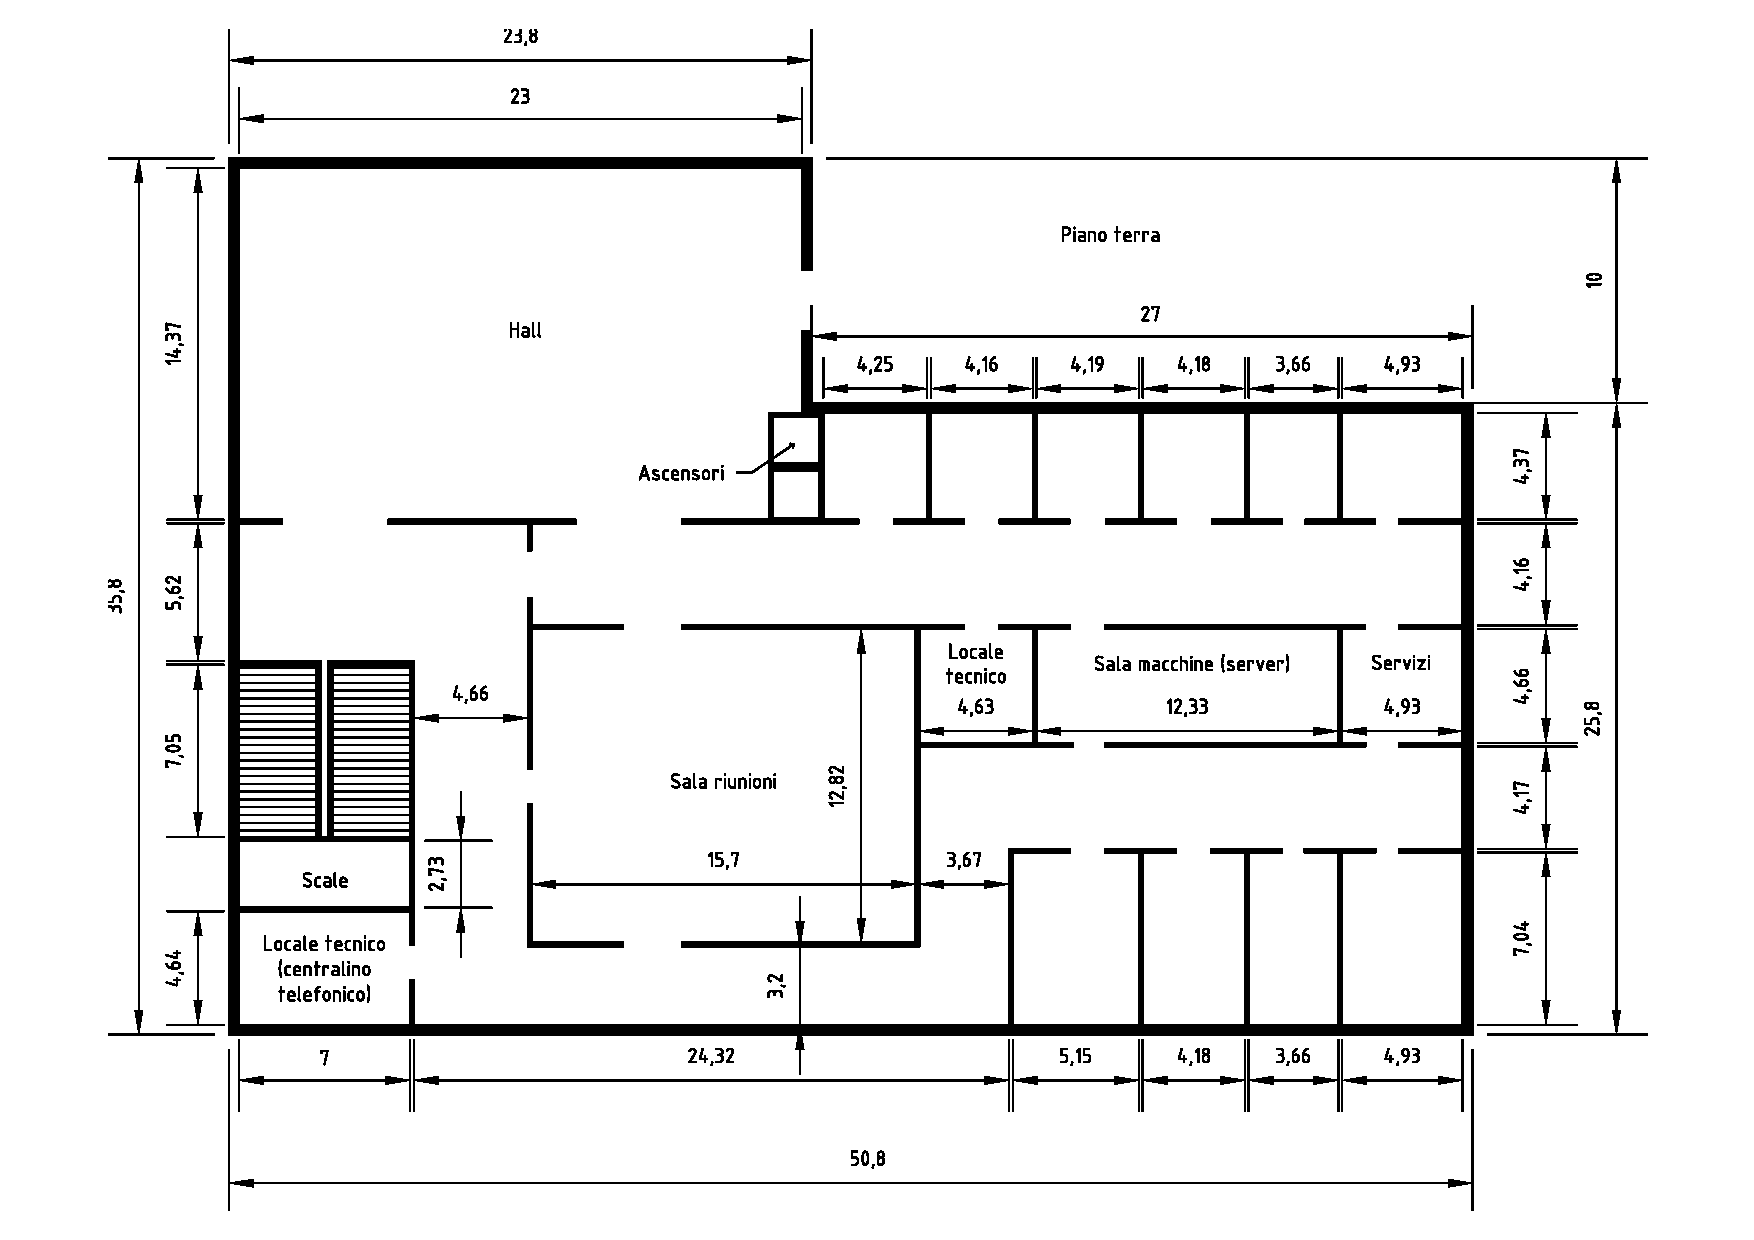
\includegraphics[width=\textwidth]{planimetrie-pianoterra}
    \caption{Planimetria del piano terreno.}
    \label{fig:planimetria-terreno}
\end{figure}

\begin{figure}[ht]
    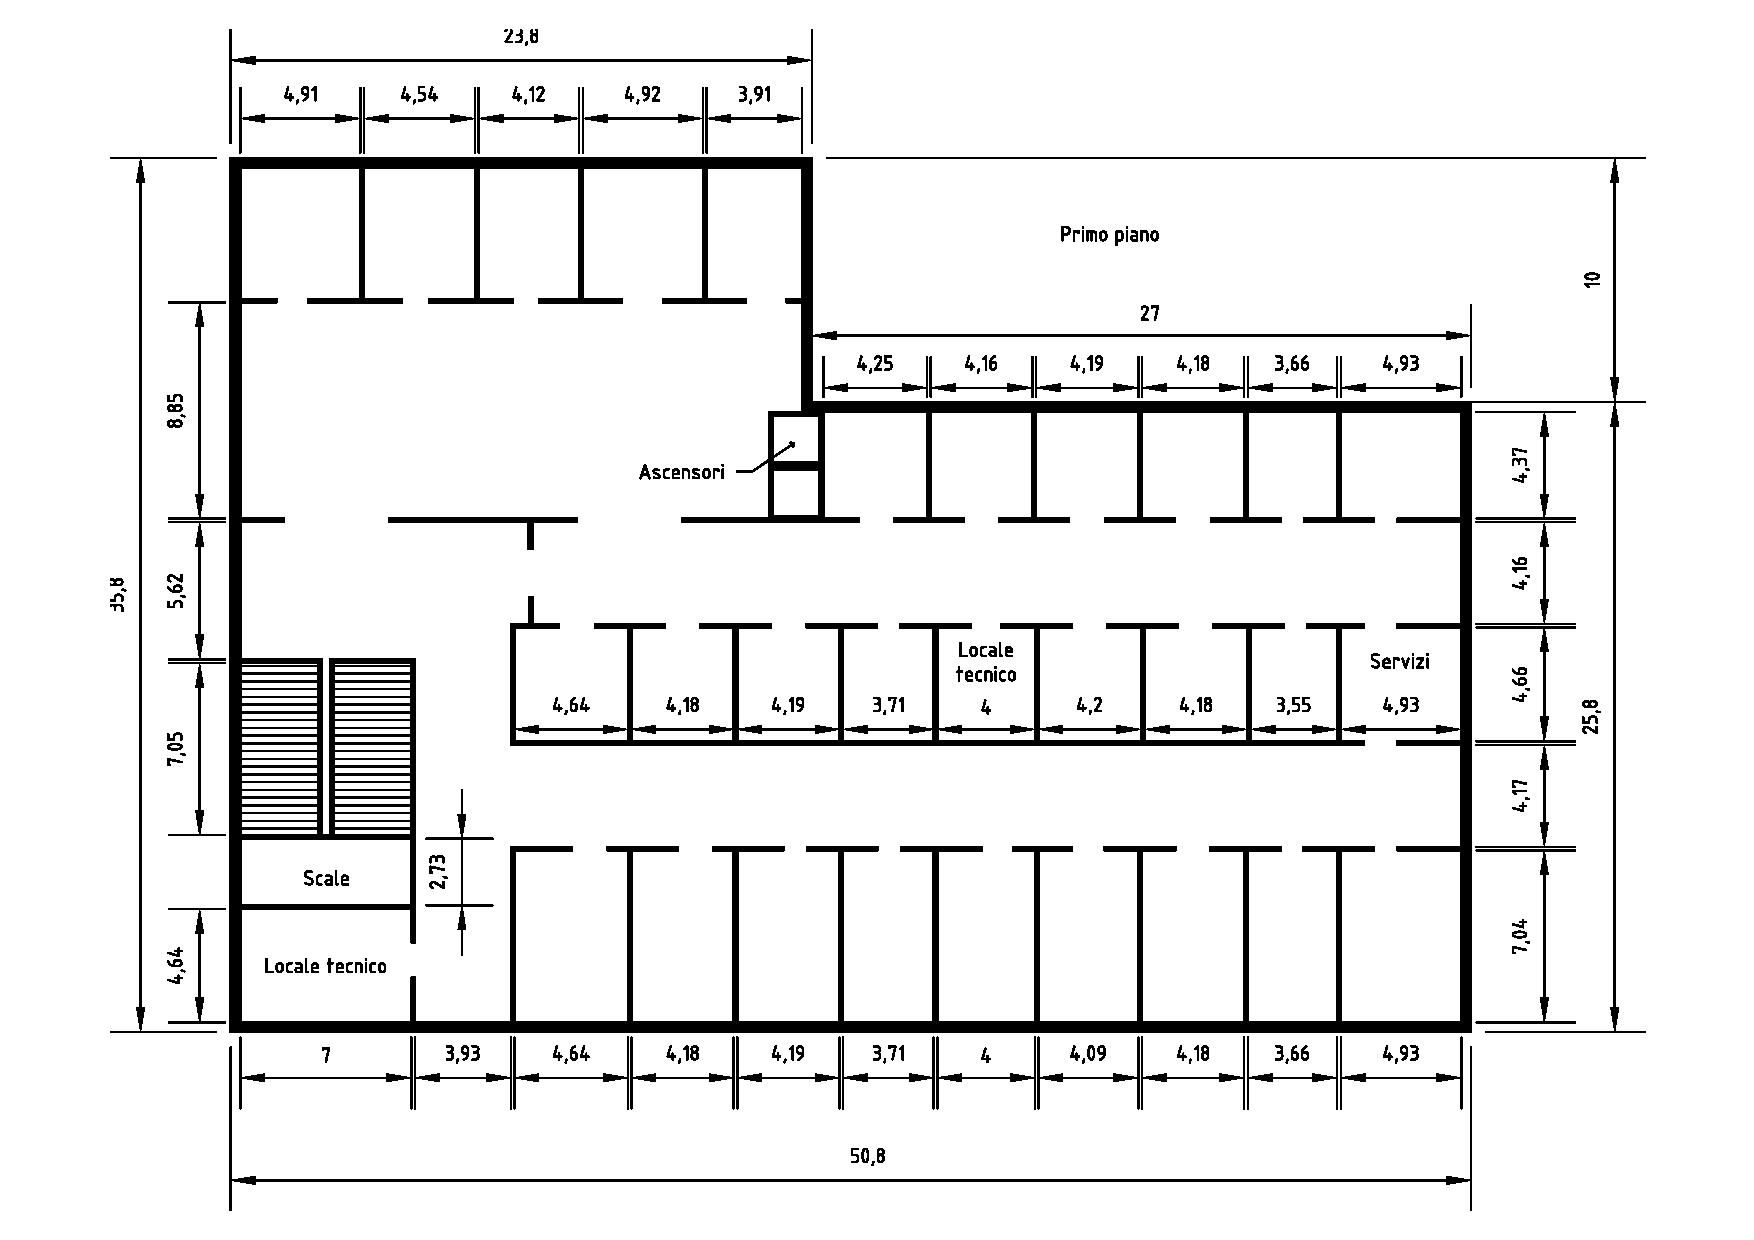
\includegraphics[width=\textwidth]{planimetrie-piano1}
    \caption{Planimetria del primo piano e dei successivi.}
    \label{fig:planimetria-1}
\end{figure}

\newpage
\section{Requisiti}
È richiesto un cablaggio standard ISO/IEC11801 con \num{2} prese in rame per ogni posto di lavoro.
In aggiunta alla topologia stellare è richiesta l’introduzione di collegamenti in rame (almeno \num{4} cavi da \num{4} coppie)
tra gli armadi adiacenti, per la realizzazione di reti fisiche di estensione limitata in piccole zone dell’edificio
e per eventuali cammini ridondanti per soluzioni fault tolerant.
Uno dei locali dell’edificio (adeguatamente indicato nelle planimetrie) dovrà essere adibito a sala macchine e
ospiterà i server.
Un centralino telefonico sarà ospitato nel vano al piano terreno che ospiterà anche l’armadio di centro stella di
edificio; in tale vano arriveranno i collegamenti ai servizi esterni.
